\documentclass[a4paper,11pt]{kth-mag}
\let\ifpdf\relax
\usepackage[T1]{fontenc}
\usepackage{textcomp}
\usepackage{lmodern}
%\usepackage[latin1]{inputenc}
\usepackage[swedish,english]{babel}
\usepackage{modifications}
\usepackage{amsmath}
\usepackage{ifpdf}
\usepackage[breaklinks=true]{hyperref}
\usepackage{breakcites}
\usepackage{pdfpages}
\newcommand{\textunderscript}[1]{$_{\text{#1}}$}
\usepackage[utf8]{inputenc}
\usepackage{cite}
%\usepackage{biblatex}
%\addbibresource{references.bib}
\newenvironment{italicquotes}
{\begin{quote}\itshape}
{\end{quote}}
\usepackage{graphicx}


%\usepackage{appendix} 
\title{Balancing Cube (working title)}
\subtitle{Stabilization and design of reaction wheel based inverted pendulum. --?-- Control and design of reaction wheel balanced inverted pendulum}
\foreigntitle{Stabilisering med svänghjul Utevkcla...}
\author{Mikael Sjöstedt \\ Alexander Ramm}
\date{May 2015}
\blurb{ Bachelor's Thesis in Mechatronics \vspace{1em} \\
\begin{tabular}{ll} 
Supervisor: Daniel Frede &  \\
Examiner:Martin Edin Grimheden \\ 
Approved: & TBA 2015-month-day
\end{tabular} }
\trita{TRITA xxx yyyy-nn}


\begin{document}

%
\includepdf[pages={1}]{kth-cover.pdf}
\clearpage

\frontmatter
\pagestyle{plain}
%\removepagenumbers
\pagenumbering{roman}
\maketitle
\selectlanguage{english}
\begin{abstract}
\addcontentsline{toc}{chapter}{Abstract}
Robots that moves requires a high degree of precision from position tracking sensors. This paper studies how the 
placement of these sensors affect the robots ability to determine its position. A robot with a cubical frame were 
built, which were able to balance on a edge with help of a reaction wheel. The robot could determine its rotation using a sensor type called --inertial measurement unit--. Different sensor positions were evaluated empirically and...
 
\end{abstract}
\cleardoublepage
\begin{foreignabstract}{swedish}
\addcontentsline{toc}{chapter}{Sammanfattning}
Robotar som förflyttar sig kraver mycket precis nogrannhet från sina positionerings sensorer. Det här rapporten tar
upp hur placeringen av dessa sensorer påverkar robotens förmåga att bestämma sin position. Från en kubformad ram 
byggdes en robot, som med hjälp av ett motordrivet svänghjul kan applicera ett internt moment för att balansera på en kant. Roboten använde en sensor av typen --inertial measurment unit-- för att bestämma sin position. Olika placeringar av sensorn utvärderases empiriskt och ...
\\


%Examensarbetet skrivs på engelska och har alltid både en svensk och en engelsk sammanfattningssida. Denna skrivmall, som inte har ``bookmarks'' eller några avancerade ``features'', definierar layouten för ett examensarbete i Maskinteknik (MF123X) eller Industriell ekonomi (MF105X).
%I detta kapitel sammanfattas examensarbetet. Sammanfattningens omfattning är högst en sida. Sammanfattningen åtföljs av en blank sida. Den föregående titelsidan, som lämpligen också innehåller en illustrativ bild, följs också av en blank sida. Alla kapitel börjar längst upp på en högersida, dvs på ett udda sidonummer.
\end{foreignabstract}
\clearpage
\chapter*{Preface}
\addcontentsline{toc}{chapter}{Preface}
Here goes our thanks to sources of  help, cooperation, inspiration \\ To be filled in \\
% Here goes credits to Daniel Frede, Staffan, Assarna som tog sig tid, eventuella maskiner som inte strulat
\begin{flushright}Alexander Ramm \\Mikael Sjöstedt \\ KTH, månad, 2015 \end{flushright}


%\clearpage


\cleardoublepage
\addcontentsline{toc}{chapter}{Contents}
\printindex
\tableofcontents*

\cleardoublepage
\chapter*{Nomenclature}
\addcontentsline{toc}{chapter}{Nomenclature}
\section*{Symbols - needs restructure}
\noindent{}\begin{tabular}{@{}p{2.5cm}l}
\textbf{Symbol} 	& \textbf{Description} \vspace{.5em} \\
$E$ 		& Elasticity module (Pa) \\
$r$		& Radius (m) \\
$t$		& Thickness (m) \\
$\mathcal{L}$			& Lagrange \\
$\theta$		& Cube angle\\
$\phi$		& Flywheel angle \\
$q$			& Lagrange operator \\
$E_k	$		& Kinetic energy \\
$E_p$		& Potential Energy \\
$I_c$		& Inertia of the cube\\
$I_f$		& Inertia of the flywheel\\
$M\textsubscript{tot}$		& Total mass of the cube\\
$M_f$		& Mass of the flywheel \\
$i$			& Current\\
$K_t$		& Motor torque constant\\
E\textunderscript{emf} 	& Induced voltage \\
K\textunderscript{emf} 	& Motor voltage constant \\
U			& Voltage across motor poles\\
$R_m	$		& Motor internal resistance \\
$\eta_m$		& Motor efficiency\\	
$\eta_g$		& Gear efficiency \\
$u$			& Gear ratio\\
$z$			& Measurement noise \\
$w$			& Process noise \\

\end{tabular}
\clearpage

\section*{Abbreviations}
\noindent{}\begin{tabular}{@{}p{2.5cm}l}
\textbf{Abbreviation} 	& \textbf{Description} \vspace{.5em} \\
CAD			& Computer Aided Design \\
CAE			& Computer Aided Engineering\\
PLM			& Product Lifecycle Management\\
PWM			& Pulse With Modulation\\
DOF			& Degrees of freedom\\
MEMS			& Microelectromechanical Systems \\
MATLAB		& Matrix Laboratory, computational program\\
RMS			& Root Mean Square\\
MCU			& Microcontroller\\
IC			& Integrated circuit\\
$I^2C$		& Inter-Integrated circuit\\
USB			& Universal Serial Bus \\
UAV			& Unmanned Aerial Vehicle\\
\end{tabular}
\cleardoublepage

\mainmatter
\pagestyle{newchap}

\chapter{Introduction}
This chapter describes the background, purpose and scope of this project conducted at the mechatronics department at the Royal Institute of Technology, KTH, Sweden. The work was carried out during the spring 2015.

\section{Background}
A reaction wheel is a wheel that is accelerated to apply torque to something. The most wide spread use of reaction wheels is in human made satellites. The  reaction wheels, usually three of them in the case of satellites, are used to change the attitude of the satellite by applying torque in a favourable manner. This is imperative to direct solar panels towards the sun or pointing antennas to assure maximum performance and connectivity to the satellite. Compared to most machines satellites are quite uncommon (there are ~1100 satellites currently in orbit [source]), and their technology can at times seem alien. But reaction wheels should not be alienated, they can be used in many contexts and this paper will cover one of them.  

Balancing 1 \textit{degree of freedom} (DOF) inverted pendulum type structures using reaction wheels is no
new concept, and became more accessible with the introduction of cheap microcontrollers.
The use of automated control is growing in a rapid pace and is being implemented
more and more in consumer related products.  This growth
has made automated control together with sensors available more now than ever. It can be seen in the every-day life in product lines such as mobile phones, gaming controllers, cars and UAV’s such as quadrocopters.

One of the most basic systems that requires some control to become stable is the inverted pendulum. 
Although it is simple to define controlling it is not a trivial task. A lot of work has been done on the topic
but there are still no knowledge easily acquired by the public available. 

The method to achieve balance of the pendulum using reaction wheels is even more narrow. 
The use of reaction wheels to change the rotation is commonly used in satellites. The exact control is also required. --SKRIVS 2 GGR--
In recent years prototypes of land based structures using reaction wheels have been a hot topic and the cubli is truly remarkable.

It would be a great achievement to contribute knowledge about how such a mechanism could be built and evaluate
the capabilities and restrictions of such a machine, on a level that does not require a PhD.


\section{Purpose}
The goal of the project was to build a structure that in one degree of freedom that can maintain balance using a reaction wheel and examine the behaviours of the system.
The behaviour (samma ord igen) is mostly effected by the control system, which is responsible for accelerating the motor in the  correct angular direction, to maintain balance. The parameters in the control system effects response time, overshoot and sinusoidal settling time.
This project will hopefully contribute to some development within the open-source community.
All results are available online, open source (MIT license reference here), on GitHub (GitHub link here).
As a mechatronical thesis, this paper can be divided into two parts. One engineering part which focus is to implement knowledge in mechanics, electronics and control theory to result in a functioning robot. And then a research part which topic could be concentrated to a question 

\begin{italicquotes}
How does the sensor placement effect the quality of the sensor data.
\end{italicquotes}
The only sensor that can be placed arbitrarily in the system is the \textit{Inertial Measurement Unit} (IMU). Certain positions might have an advantage in terms of how usable the raw data is. The IMU is a sensitive devise and disturbances such as high current and fast oscillations in its vicinity might ruin the data entirely.[citation PLZ]. With quality defined as the usability of the data given by the sensor.

\section{Scope}
The only sensor to be examined was the IMU. The encoder for the motor is fixed to the motor shaft and was not examined. Only a few key positions of the sensor were examined.
The effects that were looked at were the ones linked to the control system. Mainly the overshoot behaviour and the settling time of the system. Only data used for the specific control system were examined, other DOF measurements were not taken into consideration. I.e. the results may only be applicable in similar machines and not in general.
For every position the same parameters and constants were used in all systems and software. The comparisons were made in between measurements while balance was maintained and no external disturbance is applied. All measurements where taken during a limited time frame (We dont know this yet....). 

\section{Method}
The sensor was placed in the upper corner, one of the side corners, between the mentioned corners and in the center of the cube (insert figure reference). Both raw data and filtered data were collected and sent over serial to a computer. Using Matlab \cite{MATLAB:2014} the readings where analysed for stablization behaviour. Other obvious observations were noted. To have equal conditions, all measurements were made on the same horizontal space with the same external voltage supply.

\chapter{Theory}
This chapter cover some theory that is required if one want to build a similar robot. It is assumed that the reader has some understanding of Newtonian mechanics, signal analysis and control theory. Basic understanding of DC motor operation is also an advantage.

The first part is about the inertial reference unit that covers issues of sensor characteristics and why they are important to the system as a whole and the research question in particular.

There is a part that discuss Kalman filter theory, a filter required for getting high quality data from the IMU. The filter interprets noisy data from the sensor and digitally filters the signal to a more trustworthy output. 

The last part will cover the theory of the mechanical system behaviour that is used to develop the state space control system. The equations are responsible for the actual balance part and thus important. 

% When using a sensor such as an IMU one can choose between different resolution settings, depending of the specific usage. Although the resolutions were not changed between measurements these settings could be important when comparing to another machine


\section{Inertial Measurement Unit}
The data collected for calculating the angle of the cube is gathered from an IMU. This is an unit that uses both an accelerometer and a gyroscope to track the orientation and position. An IMU is often rated for several degrees of freedom, a unit specified as 6-DOF uses three orthogonal accelerometers and gyroscopes. These measures linear acceleration and angular velocity in each direction seperately. There are also units that are rated for additional degrees of freedom that usually includes features such as magnetometer or barometer sensors.   
To understand the fundamentals of an inertial system a cartesian coordinate system is defined
\\ \\
\textbf{Carteesian coordinate system pic here}
\\ \\

The inertial navigation system used in this project is a small \textit{microelectro-mechanical system} (MEMS). A micromechanical sensor is more or less a very small unit that take use of its mechanical properties to sense alteration in the environment \textsc{Source} . The advantages of these small units are low production costs, small size and low power consumption. As the research of these fairly modern units continues the reliability increases but they still hold a disadvantage versus the optical units that is accuracy. \cite{IMUintro}
\subsection{Accelerometer}
Accelerometers are used to measure transversal acceleration. Or rather, the device measure forces due to acceleration. These forces can be divided into two groups 
\begin{itemize}
\item Static forces, such as gravity
\item Dynamic forces, due to movement
\end{itemize}
The force is then converted to an acceleration, this is done by measuring the change in capacitance when a spring mass system is moving. The typical accelerometer consists of a movable mass that is attached via a mechanical spring or suspension system to a frame that is used as a reference. 
\\ \\
\textbf{capacitance accelerometer pic here}
\\ \\
The change of capacitance is converted to a voltage that is sent to the microcontroller for further use. The typical noise sources in an accelerometer is mechanical vibration of the springs, the circuitry and the measurement as well. These noise terms can be characterized by a white noise. Relevant for this project is how this noise effects the integrated value which is represented by the \textit{velocity random walk} (VRW). The accelerometer also outputs a constant bias, it is essential to determine the bias when estimating a position with the help of an accelerometer.
\cite{ref:accelerometero}

\subsection{Gyroscope} \label{gyroscope}
Gyroscopes unlike accelerometers, does not measure transversal acceleration. Gyroscopes, or gyros as they are referred as in everyday speech, measure the angular rate of velocity. This is done by making use of the Coriolis effect to measure the angular rate.
\\ \\
\textbf{Gyroscope pic here}
\\ \\
A mass is vibrating along an axis, with the momentary velocity $v$, and when the mass is rotated, a secondary perpendicular vibration is induced which is explained by the coriolis force
\begin{equation}\label{eq:coriolis}
\textbf{F}_c = -2m(\textbf{\textit{w}} \times \textbf{\textit{v}})
\end{equation}
The result is a physical displacement due to the Coriolis force and a capacitance is measured just like the accelerometer. So for example if a rotation occurs along the x-axis the gyroscope would output a \textit{roll} rate.

A micromechanical gyroscope is, like the accelerometer, effected by a constant bias. This is often due to friction caused by moving parts or production variations that induces stress on the construction resulting in an offset of the output. If a constant error is integrated the angular error grows linearly with time. This is easily corrected by subtracting the bias from the output.
The constant bias introduced above is not entirely constant either. The small size and sensitivity of this device is making the bias wander due to flickering noise in the electronics. Hence a \textit{bias stability} is introduced as a measurement of how the bias may change during a period of time.
More troublesome errors that occur in MEMS gyroscopes thermo-mechanical white noise similiar to the accelerometer, a more or less uncorrelated error. This can be translated to a phenomena known as \textit{Angle Random Walk} or ARW that indicates how the integrated value is effected.
The concepts of ARW, ARW and bias stability that has been introduced are more or less an indication of how precise the  are. \cite{IMUintro}  

\section{Kalman filter}
The signal from an IMU contains data of angular velocities and transversal acceleration, but also a lot of noise. An estimated position of an untreated signal from an IMU could work for short periods, but over time the estimated position \textit{drifts} \cite{MEMSdrift}. This drift occurs when measurements containing noise is integrated to acquire a position, the readings contain both white noise and often a bias which is making the  error to grow for every calulation.
Integrating the angular motion from the gyro to estimate a position would result in an angular drift and an even worse drift for the accelerometer as it is integrated twice to estimate a position.
By using a Kalman filter the drift can effectively be minimized. If the readings from both the gyroscope and accelerometer is considered, and with some help of probablity theory the estimated state is not far from the true value.  A Kalman \textit{filter} is not what the name suggests, it is an estimator. Old and new measurements are processed real-time to calculate an estimation of the current state.
Keep in mind that there are some regards that should be taken into consideration when choosing an estimator.
A good estimator produces states that are non biased, \emph{values that have an average  of the true value}. As well that the estimated state variance from the true state is as small as possible.\cite{Simon2001}


\subsection{State Estimator}
The Kalman filter is, as stated above, a state based estimator. By using the last measurement and the one before that it can derive a better estimate of the current state. The true state and the measured value at a time \textit{k} would be
\begin{equation}\label{eq:kalmanstate}
x_k = Ax\textsubscript{k-1}+Bu\textsubscript{k-1}+w\textsubscript{k-1}
\end{equation}
\begin{equation} \label{eq:kalmanmeas}
z_k = Hx_k + v_k
\end{equation}
The true state $x$ is expressed with the the old state, an input $u$, in this case data from the gyroscope. But the signal also contains a process noise $w$. The process noise $w$ in equation \eqref{eq:kalmanstate} is a representation of variances in the process that cannot be mathematically predicted. When using a gyro this reflects the error characteristics mention in section\ref{gyroscope}. 
The measured value, $z$ (see \eqref{eq:kalmanmeas}) is an observed measurement, in this case the accelerometer. Ideally this would only be a function of $x$, but is distorted by the measurement noise $v$.
The measurement noise, $v$, much like the process noise is common in any measurement and represents various fluctuations caused by the equipment.
\\ \\
As this recursive filter uses old and new values a \textit{priori} and \textit{posteriori} state is defined
\begin{equation} \label{eq: priori state}
\hat{x}^-_k
\end{equation}
\begin{equation} \label{eq: posteriori state}
\hat{x}_k
\end{equation}
The \textit{priori} \eqref{eq: priori state} state is defined as the estimate of the current state at the time $k$. The \textit{posteriori} state \eqref{eq: posteriori state} is the new estimated state.
For the Kalman filter to work properly some criteria has to be fulfilled. The average value of the measurement noise $z$ and process noise $w$ has to be zero, i.e. a Gaussian error. $z$ and $w$ also has to be independent of  each other. The noise and error in an IMU and many other devices have the charecteristics of gaussian noise.

\subsection{The process} 
The Kalman filter loops two stages. The \textit{predict} and \textit{update} stages.
\begin{figure}[!htb] 
\centering
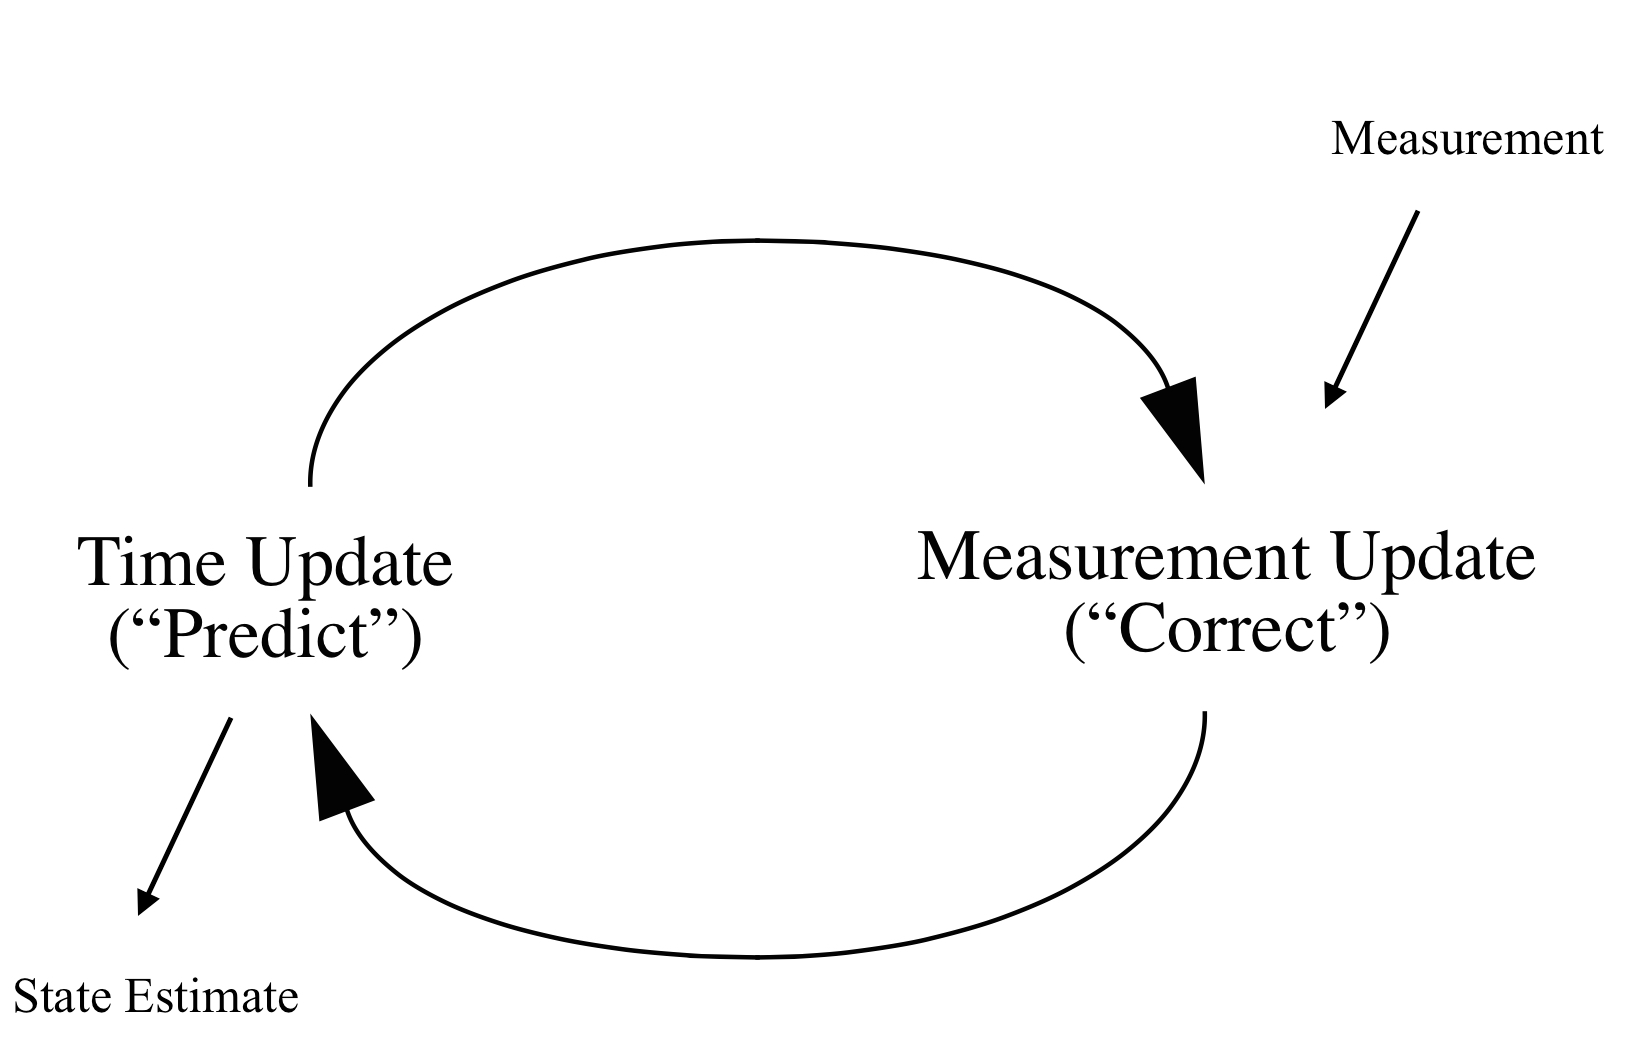
\includegraphics[width = 0.7\textwidth]{Kalmanphasepic.jpg}
\caption{Kalman phases.}
\label{figure : Kalman phases}
\end{figure}
\\ During the \textit{predict} phase the filter estimates the states using the inputs from the process, i.e the gyroscope. It then moves on to the \textit{update} phase where it compares the state to the measurement, the accelerometer. See figure \ref{figure : Kalman phases}
\begin{equation} \label{eq:Kalman first estimate}
\hat{x^-_k} = A\hat{x}^-\textsubscript{k-1}+Bu\textsubscript{k-1}
\end{equation}
As stated above the Kalman filter uses readings from both the gyroscope and accelerometer to estimate a position closer to the true value. To determine how reliable the process and measurement readings are a noise covariance is defined as
\begin{equation} \label{eq:covariance process noise}
Q = E(w_k w_k \textsuperscript{T})
\end{equation}
\begin{equation} \label{eq:covariance measurement noise}
R = E(v_k v_k \textsuperscript{T} )
\end{equation}
How to determine these covariances are further investigated in section  \ref{chapter:Allan Variance}
From here a \textit{priori} error covariance matrix is introduced to symbolize the noise in the process measurement
\begin{equation}
P^-_k = AP^-1\textsubscript{k-1}A^T + Q_k
\end{equation}
During the \textit{update} the accelerometer values are used. The measurement \textit{innovation} is calculated as
\begin{equation}
\tilde{y} = z_k - H\hat{x}^-_k
\end{equation}
The \textit{innovation} is a residual that reflects the relation between the predicted measurement and the actual measurement. A measurement \textit{innovation} of zero indicates a perfect agreement.
The measurement \textit{innovation} covariance is calculated as
\begin{equation}
S_k = HP^-_kH^T + R
\end{equation}
The \textit{innovation} covariance is very similiar to the \textit{priori} error covariance but represents the measurement instead. From here the core of the Kalman filter can be calculated, the Kalman gain
\begin{equation} \label{eq:Kalman gain}
K_k = P^-_kH^TS\textsuperscript{-1}_k
\end{equation}
indicates how reliable the measurement is. Note that if the measurement covariance error \eqref{eq:covariance measurement noise} is large the Kalman gain will be small and vice versa if the \textit{priori} error covariance is large.
By now the \textit{posteriori} state can be estimated by
\begin{equation}
\hat{x}_k = \hat{x}^-_k + K_k\tilde{y}_k
\end{equation}
A current state has been estimated and the Kalman filter returns to the measurement phase seen in figure \ref{figure : Kalman phases}.
For further reading, and mathematical proof see \cite{Kalmanintro}.

\section{Model dynamics} \label{chapter: state space}
To create a state-space model the physical model has to be translated to a mathematical model. The system can be estimated much like an inverted pendulum two-degree-of-freedom model \cite{KTHpendulum}.
\begin{figure}[!htb]
\centering
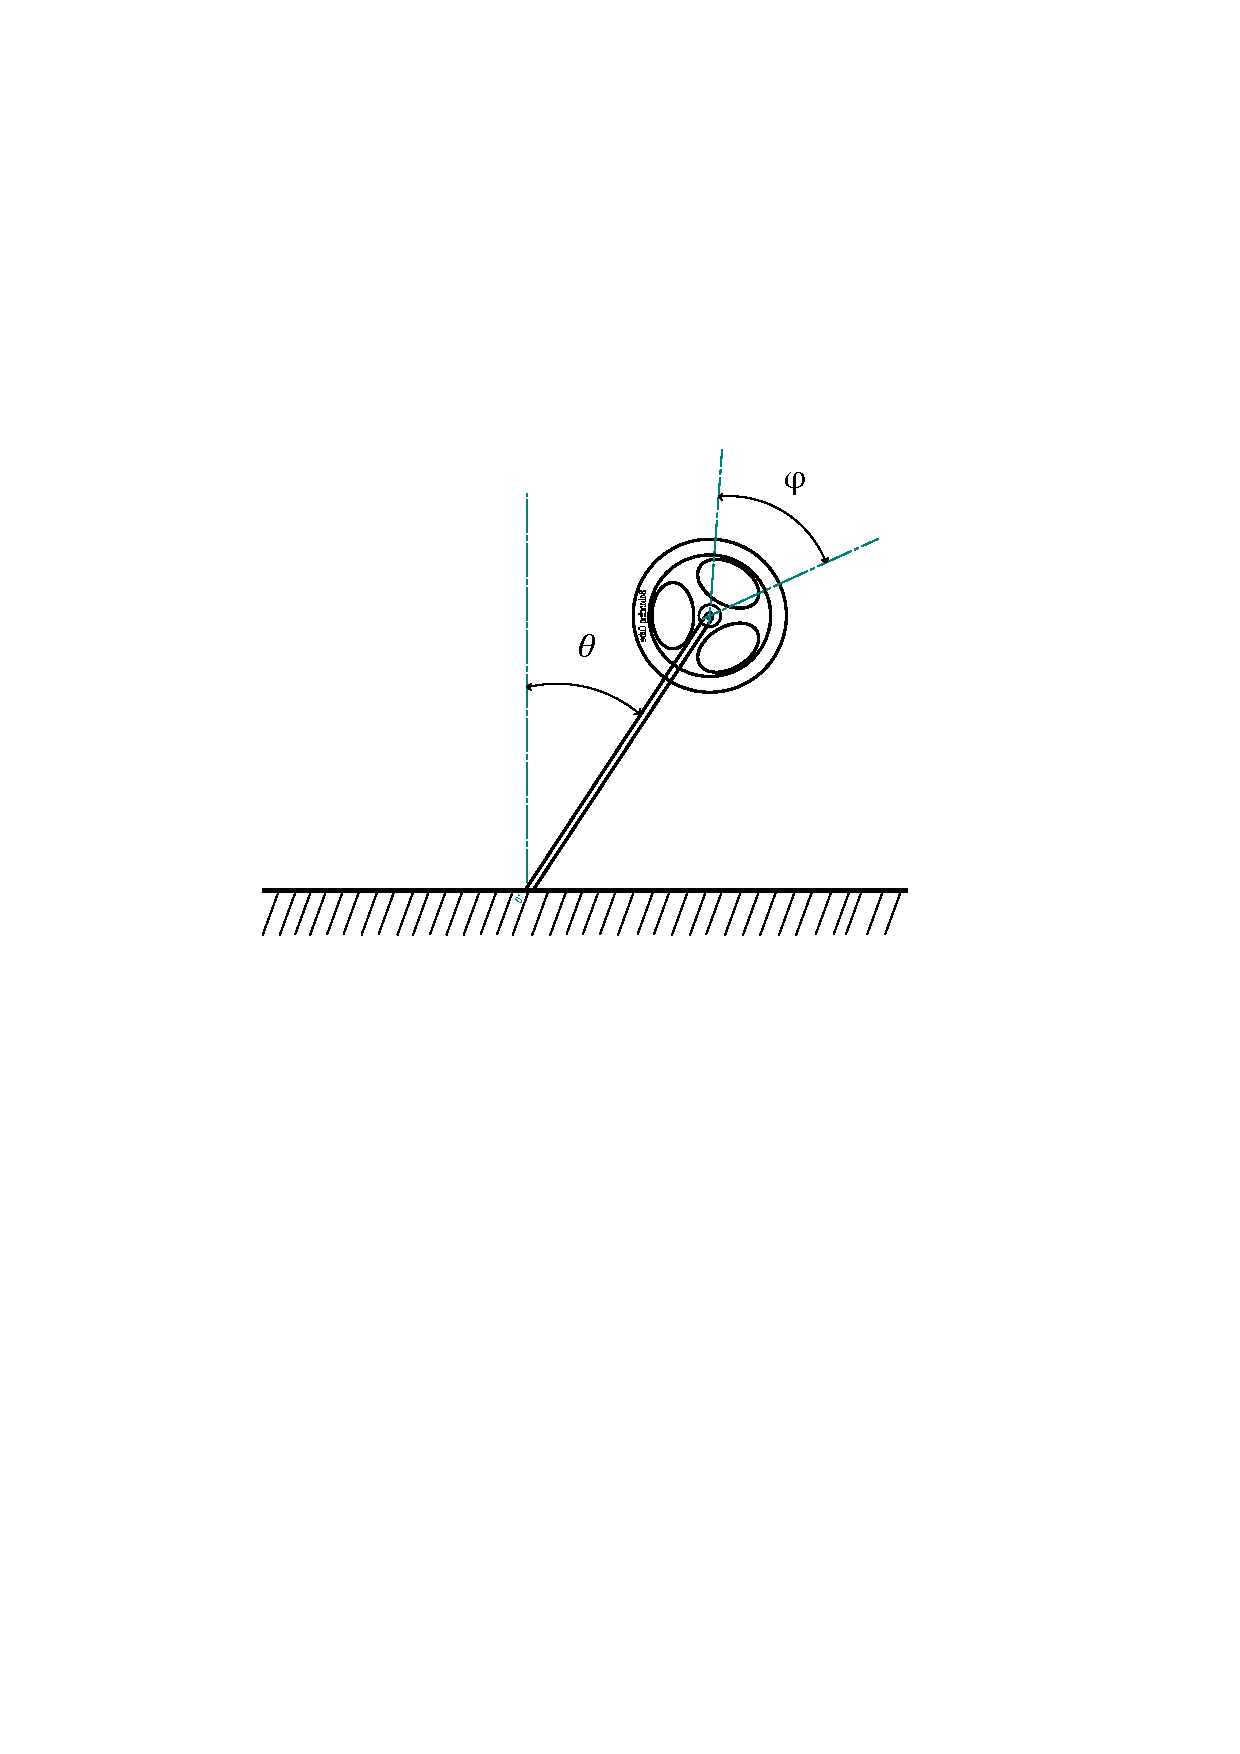
\includegraphics[scale=.6]{Lagrangeflywheel.pdf}
\caption{Cube modelled as a reaction wheel pendulum}
\label{fig:Lagrangeflywheel}
\end{figure}

\emph{Lagrangian} Dynamics have been used to derive the systems behaviour. Firstly by expressing the generlized forces, the energy functions and lagrangian. And then acquire the equations of motion from the Lagrange equation  \cite{Lagrangeref}. Consider the Lagrangian

\begin{equation}
\tau_i=\frac{d}{dt}\left(\frac{\partial L}{\partial \dot{q_i}}\right)-\left(\frac{\partial L}{\partial q_i}\right)
\end{equation}

Where $\tau$ is generilzed force, in this case a torque. The cube's angular momentum is counteracted by the flywheel and the system can be divided into two parts, One considering the movement of the cube, the other the flywheel.

\begin{equation} \label{eq:positiveL}
\tau_k=\frac{d}{dt}\left(\frac{\partial L}{\partial \dot{\theta}}\right)-\left(\frac{\partial L}{\partial \theta}\right)
\end{equation}

\begin{equation} \label{eq:negativeL}
-\tau_k=\frac{d}{dt}\left(\frac{\partial L}{\partial \dot{\phi}}\right)-\left(\frac{\partial L}{\partial \phi}\right)
\end{equation}

Whereas $\theta$ represents the angle of the cube and $\phi$ is the position of the flywheel. \\
The Lagrange equation is derived from the difference in kinetic energy and potential energy of the cube

\begin{equation} \label{eq:Lagrange}
\mathcal{L} = E_k - E_p
\end{equation}

\begin{equation} \label{eq:kinetic energy}
E_k = \frac{I_c \cdot \dot{\theta^2}}{2} + \frac{I_f \cdot \dot{\phi^2} }{2}
\end{equation}

\begin{equation} \label{eq:potential energy}
E_p = \frac{M_c \cdot g \cdot l \cdot \cos \theta}{\sqrt{2}}
\end{equation}
The lagrangian \eqref{eq:Lagrange} is then

\begin{equation}
\mathcal{L} = \frac{I_c \cdot \dot{\theta^2}}{2} + \frac{I_f \cdot \dot{\phi^2} }{2} - \frac{M_c \cdot g \cdot l \cdot \cos \theta}{\sqrt{2}} 
\end{equation}

The kinetic energy depends on the angular velocities of the cube construction as well as the flywheel fixed to the motor. Note that the total moment of inertia $I_c$ is defined around the pivot point of the cube. The potential energy has been defined as being at its maximum when the cube is balancing in an upright position. The construction is considered to be symmetric and hence the gravitational force is applied on the center of the cube.
Equation \eqref{eq:positiveL} and \eqref{eq:negativeL} with \eqref{eq:Lagrange}

\begin{equation} \label{eq:negativeL2}
I_c \cdot \ddot{\theta} + \frac{M_c \cdot g \cdot l \cdot \sin \theta }{\sqrt{2}}  = -\tau_k
\end{equation}

\begin{equation} \label{eq:postiveL2}
I_s \cdot \ddot{\phi} = \tau_k
\end{equation}

From these equations it is evident that $\tau_k$ is the torque executed on the flywheel which is wielded by the motor torque $\tau_m$, it can be described by a relation between the torque constant and the current flowing through the motor.

\begin{equation}
\tau_m = K_t \cdot i_m
\end{equation}

The current can be described by the voltage across the two poles of the motor.

\begin{equation} \label{eq:motor torque}
\tau_m = K_t \cdot \frac{U-E_{\text{emf}} }{R_m}
\end{equation}

Note that the motor inductance in neglected in equation \eqref{eq:motor torque}, that is due to the time constant which is fast considering the rest of the system and is not vital for the control system \cite{KTHpendulum}.
The induced voltage can be described as a function of motor speed.

\begin{equation}
E_{\text{emf}} = K_{\text{emf}} \cdot \dot{\phi_r}
\end{equation}

\begin{equation}
\phi_r = \dot{\phi} - \dot{\theta}
\end{equation}
 
\begin{equation} \label{eq:tau}
\tau_m = \frac{K_t}{R_m} U - \frac{K_t K_{\text{emf}} }{R_m} \dot{\phi} + \frac{K_t K_{\text{emf}} }{R_m} \dot{\theta}
\end{equation}

The torque executed on the flywheel can then be described with the torque on the motor shaft, efficiency and gearing. \textsc{Not completely finished with this part}
\begin{equation} \label{eq:eff}
\tau_k = \tau_m \cdot \eta_m \cdot \eta_g \cdot u
\end{equation}
Based on equation \eqref{eq:negativeL}, \eqref{eq:positiveL} and \eqref{eq:eff} the system can be described by
\begin{equation}
\ddot{\theta} = -\frac{K_t \eta_m}{R_m I_c} U + \frac{K_t K_{\text{emf}} \eta_m}{R_m I_c} \dot{\phi} - \frac{K_t K_{\text{emf}} \eta_m}{R_m I_c} \dot{\theta} - \frac{Mt g l }{\sqrt{2} I_c} \sin \theta \label{thetadotdot}
\end{equation}
\begin{equation}
\ddot{\phi} = \frac{K_t \eta_m}{R_m I_f} U + \frac{K_t K_{\text{emf}} \eta_m}{R_m I_f} \dot{\phi} - \frac{K_t K_{\text{emf}} \eta_m}{R_m I_f} \dot{\theta} 
\label{phidotdot}
\end{equation} 
To use linear control methods the model has to be linearised. This is done at the instable equilibrium where the cube is balancing. Consider the sinus term at the equilibrium point where $\theta$ equals $0$. The term can then be expressed with taylor/macloaruin expansion

\begin{equation} \label{eq: sinus taylor}
sin \theta = \theta - \frac{\theta^3}{3!} +\frac{\theta^5}{5!}... \approx \theta 
\end{equation}

With the equations \eqref{thetadotdot} and \eqref{phidotdot} the system can be described with a state space model with a states $x^T = [\theta, \dot{\theta}, \dot{\phi}$]. The system is hence described by
\begin{equation}
\dot{x} = Ax + Bu
\end{equation} 
where \\
\begin{center}
$\textbf{A} =\begin{bmatrix}
0 & 1 & 0 \\
-\dfrac{Mt g l }{\sqrt{2} I_c} & - \dfrac{K_t K_{\text{emf}} \eta_m}{R_m I_c} & \dfrac{K_t K_{\text{emf}} \eta_m}{R_m I_c} \\ 
0 & \dfrac{K_t K_{\text{emf}} \eta_m}{R_m I_f} & -\dfrac{K_t K_{\text{emf}} \eta_m}{R_m I_f}
\end{bmatrix}$

$\textbf{B} = \begin{bmatrix}
0 \\ 
-\dfrac{K_t \eta_m}{R_m I_c} \\
\dfrac{K_t \eta_m}{R_m I_f}
\end{bmatrix} $
\end{center}
 
\section{Control theory}
To create a state space feedback loop...
Use Ackermann instead of place? Why ?

\section{Pulse Width Modulation}
Pulse Width Modulation:
Acording to en.wikipedia.org: "Pulse-width modulation (PWM) [...] is a technique used to encode a message into a 
pulsing signal."
This is useful in many power applications, from dimming LED's to motor control. The idea of 
PWM is to alter the voltage over a device while still only having a set level voltage to supply. Simplified  
the voltage is cut into a square wave. This is done by using two transistors, one that can short the motor poles and one that distibrutes the supply voltage to be applied to the motor \cite{elektro}. If these transistors are swiched on and of fast 
compared to the time constant of the motor, the root mean square (RMS) voltage will be the acting voltage.(formel i bilaga)
This allows for a DC voltage that is percived as lower than the acual supply voltage.
They duty cycle can be changed during operation unlike liner type voltage regulators. 
 
\chapter{Demonstrator}
\emph{Detta kapitel beskriver både den utvecklade demonstratorn och den aktuella arbetsprocessen som demonstartorn utvecklats enligt, dvs resultatet och vägen dit.}
VAD FAN ÄR PROBLEMET MED MIN STATE SPACE DET KNASAR JU GRANDE WTF MODE

\section{Problem Formulation}
%Beskriv din problemställning för demonstratorn.\\

The engineering problem were to build a cube that, using a reaction wheel, could balance on its edge.
\emph{To be continued}


\section{Model validation}
To synthesize a mathematical model from a real world problem it's often beneficial to simplify the reality. Examples of assumption made for this application would be that center of mass is located at the center of the cube, the friction in the motor is ignored and the frame is considered stiff etcetera. 
To validate the model from chapter \ref{chapter: state space}, events with known results can be tested. To do so, Simulink \cite{MATLAB:2014} is used.
First of all the DC-motor model is validated to known characteristics, such as no load speed and current. 

\textbf{Graph here}
\\
The graphs in figure (ref) displays the speed and current of the unloaded motor. Showing that it   

The dynamics of the cube is simplified as an inverted pendulum. That means if there is no control input to the system it should behave as pendulum in free movement. That is, it should oscillate at a constant amplitude. As there is no torque applied to the flywheel the rotor should remain zero at all times. 
\section{Discrete Kalman filter} \label{sec: discrete kalman}
To implement the Kalman filter in an algorithm it has to be discretizied 
This is done much like a feedback control. The filter firstly? estimates the process state and then obtains feedback as noisy measurements. That means that the filter works in two steps, a \textit{time update} and a \textit{measurement update}. The names implicate that the \textit{time update} projects the next state to obtain the \textit{priori estimate} whilst the \textit{measurement update} uses the feedback mentioned above to obtain an improved \textit{posteriori} estimate.


Some of the implementation and discretization of the filter.
\subsection{Kalman implementation}
The Kalman filter cycles two states, the \textit{predict} and \textit{update} phases. Making the filter implemented on a microprocessor fairly simple. 
An implementation of the Kalman filter on the IMU would look something like this for the gyroscope





\begin{figure}[!htb]
\centering
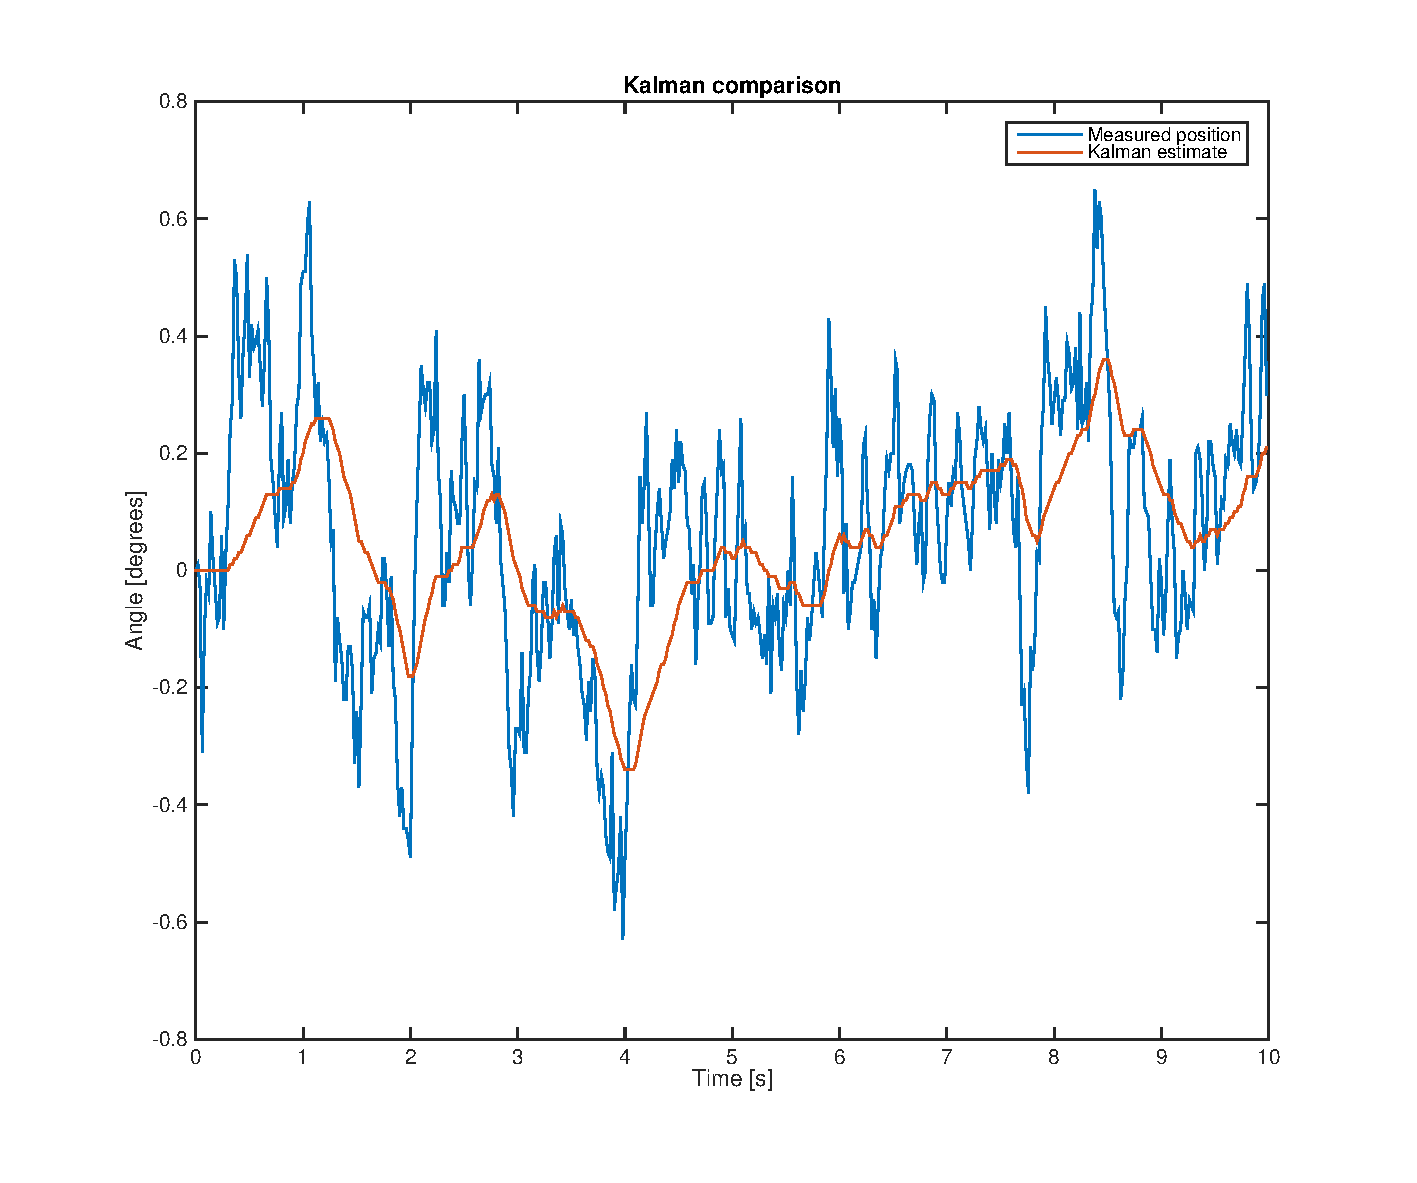
\includegraphics[scale=.7]{Kalmancomparisonplot.eps}
\caption{Comparison of Kalman filtered signal and original signal (TO BE UPDATED)}
\label{fig:Kalman comparison}
\end{figure}



\subsection{Measurement and process noise} \label{chapter:Allan Variance}
For the Kalman filter to properly work it is essential to know how reliable the process and measurement inputs are. A way of determining the process noise and measurement noise of the IMU is the Allan variance method ref.
The gyro data is treated as an external input to the system, so the error and bias from the gyro readings are characterised as process noise. This is then compared to the measurement, the accelerometer which contains a measurement noise.
More to come
% By gathering samples from the gyroscope and accelerometer at a stationary state the Allan variance can be calculated for the readings. The Allan variance is then used to determine the noise ans stability of the system. The interessting components of the variance for the IMU are angle random walk (ARW) and the bias stability, as well as the velocity random walk (VRW) for the accelerometer. The theory of Allan variance is out of the scope of this thesis but can be found --- 

\section{Software}
To develop and improve a system such as this is an iterative process. To verify changes and improvements in realtime, the model were simulated with Simulink\textsuperscript{\textregistered}. 
%\begin{figure}[!htb]
%\centering
%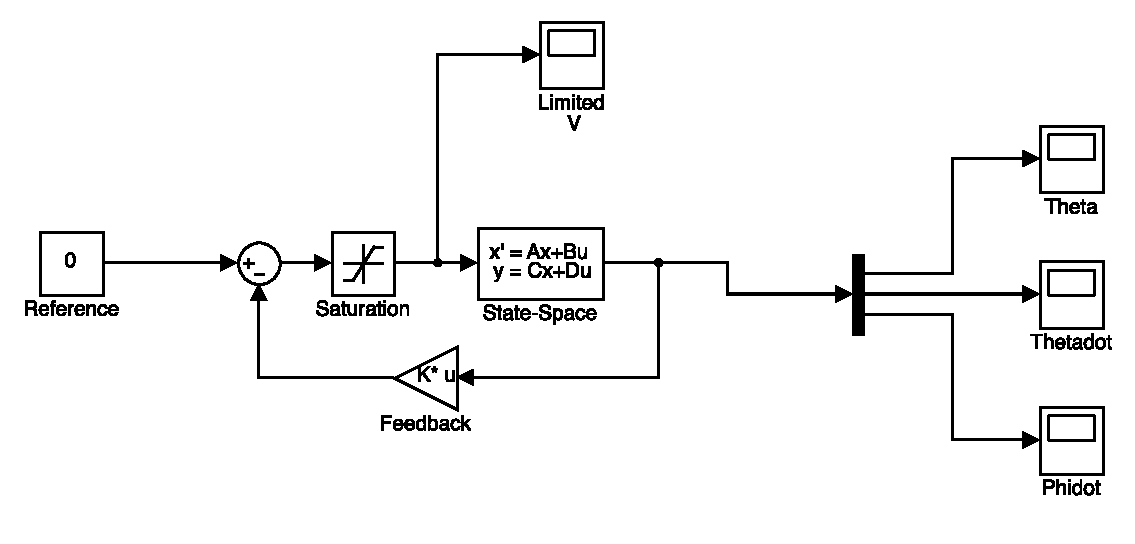
\includegraphics[scale=.7]{simmodel.eps}
%\caption{Simulink model.}
%\label{fig:simmodel}
%\end{figure}



The Simulinkmodel seen in figure \ref{fig:simmodel} describes the system
\\ Something about the  optimizing of the feedback control
\begin{figure}[!htb]
\centering
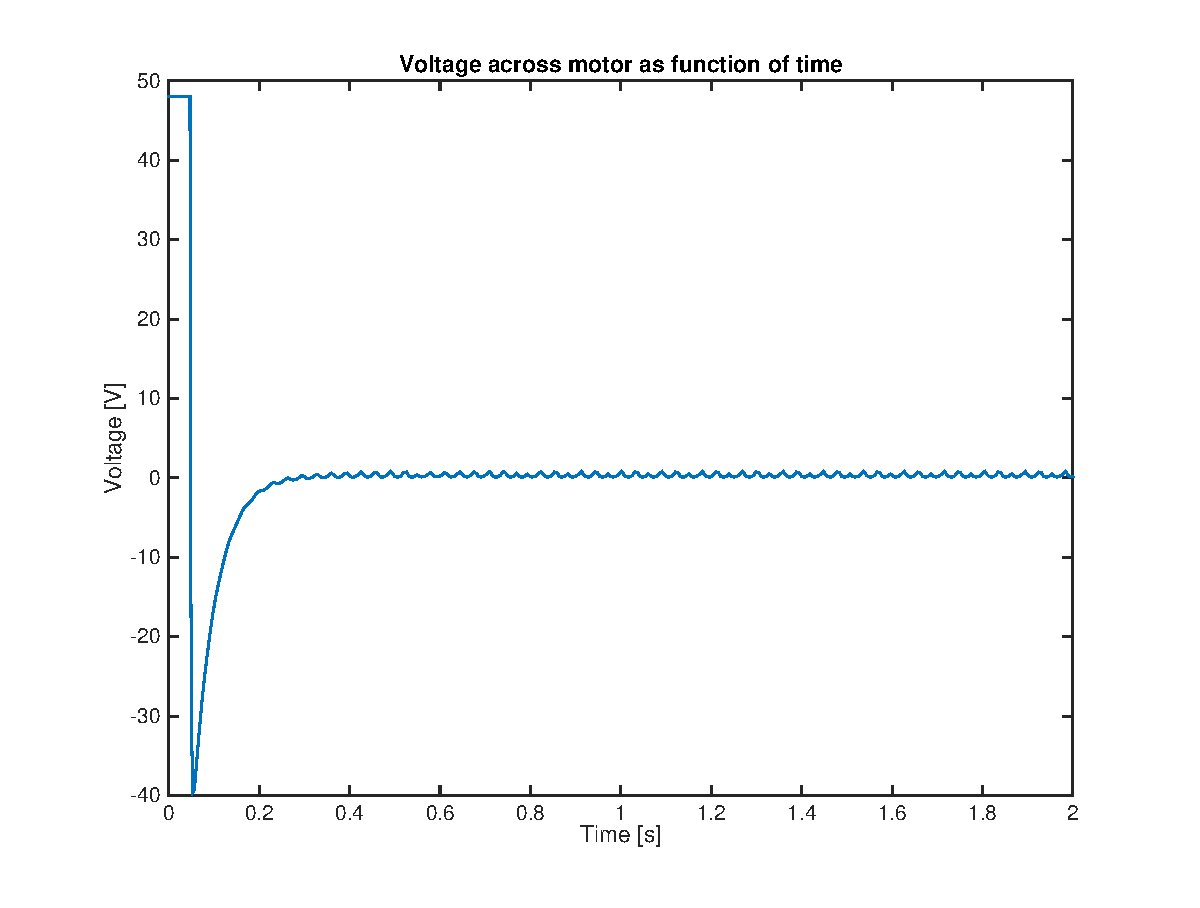
\includegraphics[scale=.7]{voltageplot.eps}
\caption{Voltage across motor poles.}
\label{fig:voltageplot}
\end{figure}

The voltage supplied to the motor

\begin{figure}[!htb]
\centering
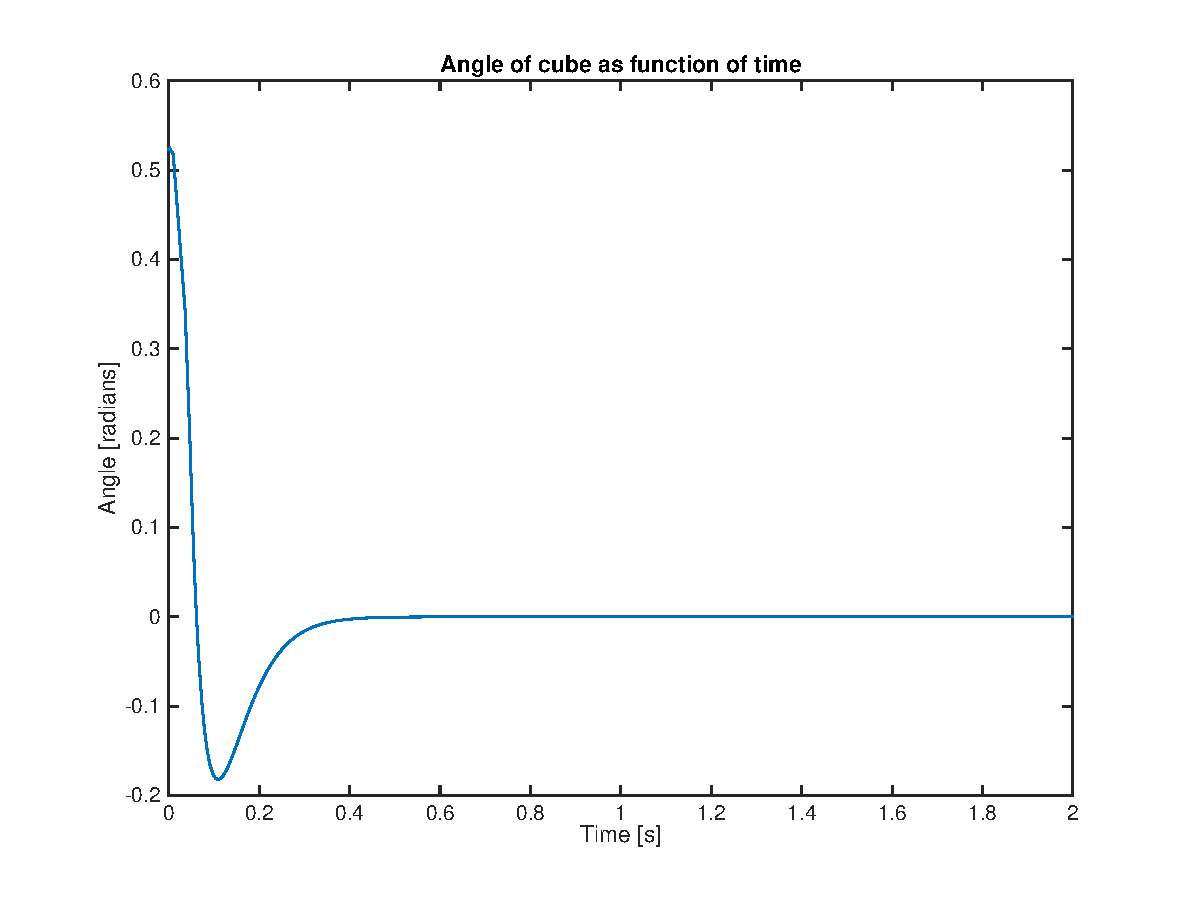
\includegraphics[scale=.7]{angleplot.eps}
\caption{Angle of the cube.}
\label{fig:voltageplot}
\end{figure}

The angle of the cube. Very good such magic


\section{Electronics}
Beskriv din elektroniska konstruktion. Använd figurer och förenklade blockschema. Motivera dina lösningar.
How do we send data?
\\ Sensors
\\ Motor
\\ Arduino
\\ Motor control

\subsection{PWM}
skriv lite om PWM hax

\section{Hardware}
The motor is fixed through the middle wall in the cube, the shaft on one side and the body on the other. The flywheel is dicrectly mounted to the motor shaft. All other components are mounted on the motor-body side of the cube.
\\ Basic construction



\section{ALLT NEDANFÖR ÄR FRÅN METHOD SÅ GÖR VAD FAN MAN VILL MED DET HÄR PAJSDÅOAIHSDAIOHUSD}

%Den metod eller de metoder, som huvudsakligen används för att angripa den uppgift eller det problem som definieras ovan, kan antingen definieras i introduktionskapitlet eller förklaras mera ingående i ett följande metodkapitel.\\

The engineering task The main goal of this project was to build a structure which remain stable in an unstable condition. A process of this sort can be divided into several parts. 
\begin{itemize}
\item Construction
\item Motor Control
\item Sensor Reading
\item System Control
\item Final Assembly
\end{itemize}

\section{Construction}
The main construction problem where deciding the size of the cube and reaction wheel. A too big reaction wheel for the motor has a large affect on the cubes ability to balance. The problem were (uppställt) with Newtonian mechanics.
Also idealy the cube should be nice looking, easy to produce and simple to assemble. 
 
\section{Motor and Motor Control}
The motors nominal and stall torque are very important for the system blaha. The motor driver is also important, but usually one can get suggestions on drivers from motor manufactures, which was the chosen path.
  
\section{Sensor Reading}
The IMU's parameters and filtering of the signals

\section{System Control}
The choosen control method where state space. The problem in to linareise and discretise with good enough precition.

\section{Final Assembly}
When the subproblems above are solved and constructed, the final machine can be built. Here cabling and disturbances from other subsystems must be taken into consideration. 
The IMU placement would provisoricly be tried to se a placement were bad due to more disturbances form other compunents i.e. netsupply and motor lining.

\chapter{Results}
Beskriv resultatet. 

\chapter{Discussion and conclusions}
\emph{I detta kapitel diskuteras och sammanfattas de resultat som presenterats i föregående kapitel. Sammanfattningen baseras på en resultatanalys och syftar till att svara på den fråga eller de frågor som formuleras i kapitel i.}

\section{Discussion}
Motor choice osv

\section{Conclusions}
Successful victory


\chapter{Recommendations and future work}

\section{Recommendations}
A more extensive research with non-linear control systems has been done at ETH, with the name Cubli,\cite{cubliECC13}

\section{Future work}
An extension of the project would be balancing the cube not only on it's edge but it's corner. To achieve this multiple reaction wheels must be used and a more complicated control system due to changes in moment of inertia caused by angular velocities in the other reaction wheels.

%\bibliography
\cleardoublepage
\bibliography{FiM_references}
\bibliographystyle{elsarticle-num-names}%apalike-url}

\cleardoublepage
\appendix
\addtocontents{toc}{\protect\contentsline {part}{Appendices}{}{}}


\chapter{Additional information} \label{appA}
\section{Kalman implementation}
\textsc{Kalman implementation goes here}

Consider the equation \eqref{eq:Kalman first estimate} from theory chapter.
\begin{equation}
\hat{x^-_k} = A\hat{x}^-\textsubscript{k-1}+Bu\textsubscript{k-1}
\end{equation}


\begin{equation}
\textbf{x}_k = \begin{bmatrix}
\theta \\
\dot{\theta_b}_k
\end{bmatrix}
u\textsubscript{k-1} = \dot{\theta}
\end{equation}

\begin{equation}
\textbf{A} = \begin{bmatrix}
1  & -\Delta t \\
0   & 1
\end{bmatrix}
,
\textbf{B} = \begin{bmatrix}
\Delta t \\ 0
\end{bmatrix}
\end{equation}
\chapter{Proofs} \label{appB}

\cleardoublepage   
\cleartoverso %force back cover to be "left" page
%
\includepdf[pages={2}]{kth-cover.pdf}

%\printbibliography
\end{document}

